\section{Common Distributions}
% ======================================================================

\begin{sectionbox}
	\subsection{Binomialverteilung $\mathcal B(n,p)$ mit $p \in [0,1], n \in \N$}
	Folge von $n$ Bernoulli-Experimenten\\
	$p$: Wahrscheinlichkeit für Erfolg \qquad $k$: Anzahl der Erfolge \\
	\\
	$p_{\X}(k) = B_{n,p}(k) = \begin{cases}
	\binom{n}{k} p^k (1 - p)^{n - k} & k \in \left\{0,\dots,n\right\} \\
	0 & \text{sonst} \\
	\end{cases}$
	\\
	\everymath{\displaystyle}
	\begin{tablebox}{l@{\extracolsep\fill}ll}
		$\underset{\text{Erwartungswert}}{\E[\X] =n p}\quad $ & $\underset{\text{Varianz}}{\Var[\X] =np (1-p)}$ & $\underset{\text{Wahrscheinlichkeitserz. Funktion}}{G_X (z) = (pz + 1 -p)^n}$\\
	\end{tablebox}
\end{sectionbox}

\begin{sectionbox}
	\subsection{Normalverteilung}
		\parbox{3.3cm}{\emph{WDF/PDF:} \\ 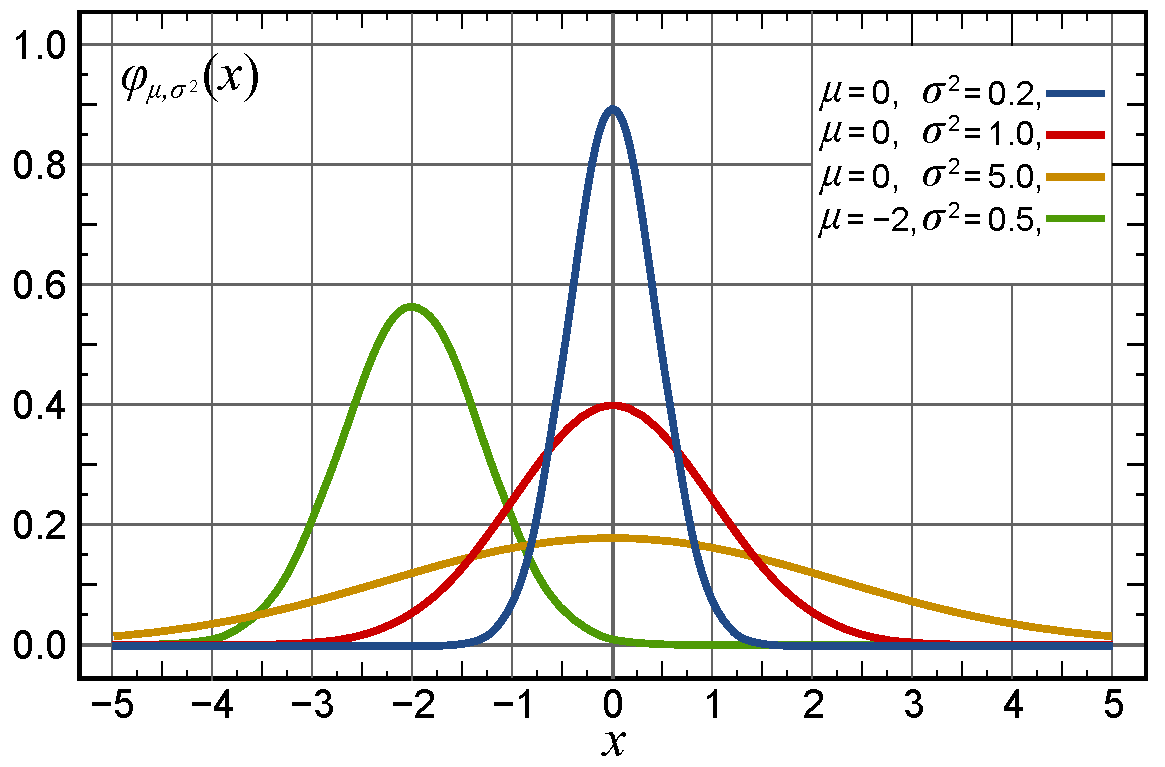
\includegraphics[width = 3.3cm]{./img/normal_pdf.pdf}}
		\parbox{3.3cm}{\emph{KVF/CDF:} \\ 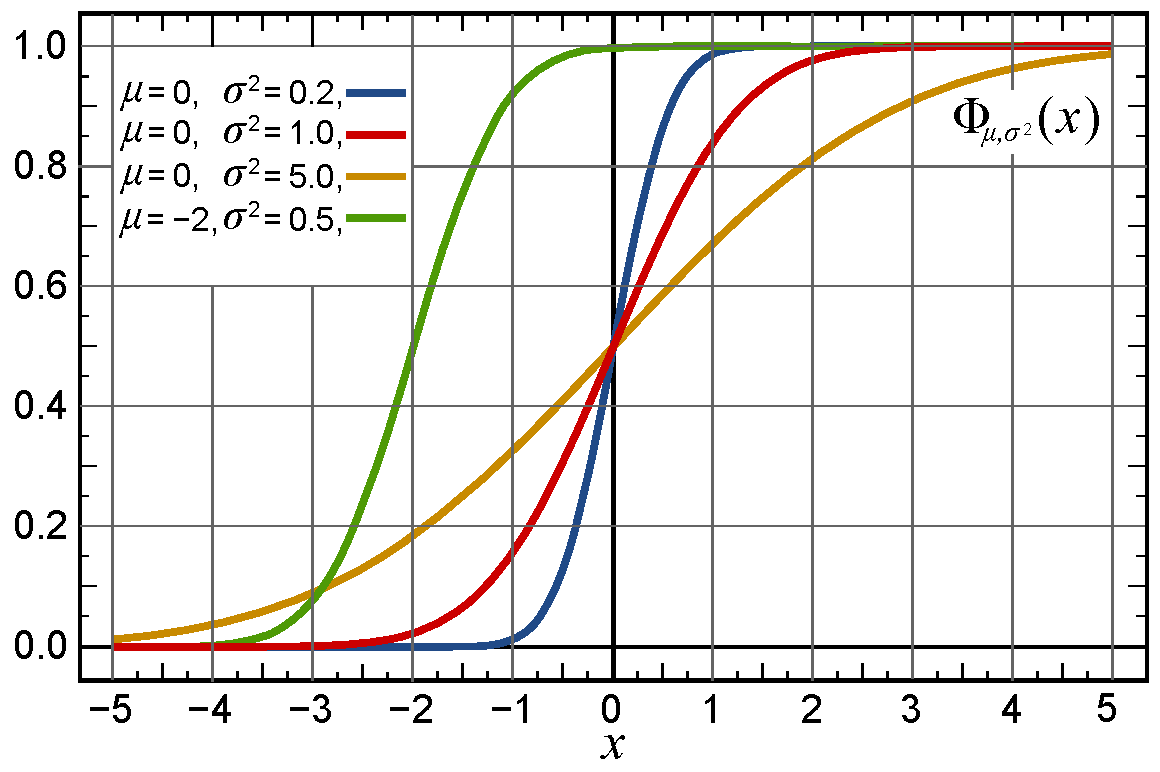
\includegraphics[width = 3.3cm]{./img/normal_cdf.pdf}}
		\textbf{WDF: }
		\boxed{f_X (x) = \frac{1}{\sqrt{2 \pi \sigma^2}} e^{-\frac{(x-\mu)^2}{2 \sigma^2}} \quad x \in \mathbb R} \qquad \parbox{1.2cm}{$\mu \in \mathbb R$ \\[0.5em] $\sigma > 0$}

		\begin{tablebox}{lll}
		\everymath{\displaystyle}
			$\underset{\text{Erwartungswert}}{\E(\X) = \mu}$ & $\underset{\text{Varianz}}{\Var(\X) =\sigma^2}$ & $\underset{\text{Charakt. Funktion}}{\varphi_{\X}(\omega) = e^{j\omega\mu-\frac{\omega^2\sigma^2}{2}}}$\\
		\end{tablebox} \everymath{\textstyle}
\end{sectionbox}

\begin{sectionbox}
	\subsection{Sonstiges}
	\textbf{Gammadistribution} $Γ(α,β)$: $\E[\X] = \frac{α}{β}$\\
	\textbf{Exponential:} $f(x,λ) = λ e^{-λx}$ \quad $\E[\X] = λ^{-1}$ \quad $\Var[\X] = λ^{-2}$
\end{sectionbox}